% Primary local LaTeX source for the revised Overleaf draft.
% The Numerical Use Case consolidates the earlier simulation and Results blocks.
% Copy this whole file into Overleaf as needed.
% Figures: upload the plot_*.png files from analyses/plots/ to the Overleaf
% project (graphicspath below also resolves them locally).

\documentclass{article}
\usepackage{graphicx} % Required for inserting images
\graphicspath{{figures/}}
\usepackage{amsmath}
\usepackage{amssymb}
\usepackage{booktabs}
\usepackage{longtable}
\usepackage{caption}
\usepackage{pdflscape}
\usepackage{placeins}
\usepackage{eso-pic}
\usepackage[backend=biber,style=authoryear,sorting=nyt,maxcitenames=2,maxbibnames=99,uniquelist=false]{biblatex}
\addbibresource{references.bib}
\captionsetup{font={small,it},labelfont={small,bf}}

\newcommand{\LandscapePageNumber}{%
  \AddToShipoutPictureFG{%
    \AtPageLowerLeft{%
      \put(
        \LenToUnit{\dimexpr\paperwidth-1cm\relax},
        \LenToUnit{0.5\paperheight}
      ){%
        \makebox(0,0){\rotatebox{90}{\thepage}}%
      }%
    }%
  }%
}

\begin{document}

\begin{titlepage}
\centering

{\large\textbf{The Hebrew University of Jerusalem}\par}
\vspace{0.35cm}
{\large\textbf{The School of Business Administration}\par}

\vfill

{\large Final Research Paper for the Degree of\par}
\vspace{0.2cm}
{\large Master of Business Administration\par}
\vspace{0.2cm}
{\large Specialization in Operations Research\par}

\vfill

{\LARGE\textbf{Evaluating Routing Rules Using Social Welfare}\par}

\vfill

{\large Submitted by\par}
\vspace{0.2cm}
{\large Yehuda Raanan\par}

\vspace{1.2cm}

{\large Supervisor\par}
\vspace{0.2cm}
{\large Professor Nicole Adler\par}

\end{titlepage}

\pagenumbering{roman}
\setcounter{tocdepth}{1}
\tableofcontents
\clearpage
\pagenumbering{arabic}

\section{Introduction}
Digital navigation systems influence the route choices of drivers sharing a road network. A routing rule converts traffic information into route recommendations. When many drivers receive similar recommendations at the same time, they may converge on the same route, causing a road that appeared uncongested when it was recommended to become congested before they arrive. Evaluating a routing rule therefore requires accounting for the traffic conditions created by the collective response to its recommendations.

Traffic and navigation research commonly evaluates routing through prediction accuracy and total driving time. Prediction accuracy asks whether the driving time forecast for a recommended route matches the time that drivers later experience, while total driving time sums the driving times experienced by all network users. Both measures treat drivers as identical because neither recognises that drivers value time differently, that tolls may alter route choices, or that a driver may forgo a trip whose expected cost exceeds its likely benefit. Prediction accuracy is also judged only on the route selected. A forecast of thirty minutes is accurate if the selected route takes thirty minutes, even when an alternative would have taken twenty minutes. An accurate forecast may therefore still provide poor route advice.

This research evaluates routing rules through a generalised cost function, which converts driving time and tolls into a single monetary figure using each driver's value of time. For every driver, the analysis compares the generalised cost expected at the moment a route is chosen with the cost eventually incurred. The gap between the two indicates whether the routing rule anticipated the congestion that its recommendations helped to create. A complementary measure, routing regret, estimates the additional cost a driver incurs when the selected route is estimated to be more costly than an available alternative.

The research evaluates individual outcomes through consumer surplus and system-level outcomes through social welfare. Consumer surplus represents the value an individual driver retains after incurring generalised cost, while social welfare combines consumer surplus across drivers with the estimated effect of public toll revenue. The System Optimum provides a coordinated allocation that maximises welfare under comparable conditions. Experienced welfare loss measures how far a routing rule falls below this benchmark while reflecting differences in value of time, decisions whether to drive, and the welfare effects of tolling. It therefore differs from the classical Price of Anarchy, which is the ratio of total driving time at User Equilibrium to the minimum total driving time under the System Optimum.

Tolling may reduce congestion by redistributing drivers between routes, reducing the number who choose to drive, or both. Some drivers may switch routes when one becomes more costly, while others may decide not to drive when the expected cost of every available route exceeds the expected benefit of the trip. Drivers who choose not to drive avoid the expected cost of driving but forgo the expected benefit of the trip, and the welfare comparison accounts for both effects.

The research examines these relationships in a controlled road-network microsimulation. The setting represents a familiar daily choice between a shorter route that may be tolled and a longer alternative. Drivers decide whether to drive and, if so, which route to use based on expected driving times and applicable tolls. Their combined choices produce the congestion they later experience. Elastic demand represents the participation decision by making the no-trip alternative more likely as perceived generalised cost increases. Holding the network, potential-driver population, and behavioural assumptions constant allows the analysis to isolate the effects of routing rules and toll levels.

The numerical use case compares three routing rules. Moving Average represents backward-looking guidance based on recently observed driving times. Forward Looking accounts for current route assignments when predicting the conditions that departing drivers may encounter. Habitual represents route choices based on fixed probabilities that do not respond to current traffic. Comparing these rules separately and within mixed populations isolates differences associated with information timing and population composition.

The research contributes a common welfare framework that links route information and collective response to experienced generalised cost, participation, consumer surplus, and social welfare. Comparisons with a System Optimum under the same toll measure the welfare loss associated with each routing rule, while a separate zero-toll benchmark decomposes welfare differences into routing-rule, toll, and mixed-population interaction contributions.

The practical significance of this research lies in the possibility that a routing rule that predicts driving time accurately or reduces total driving time may nevertheless produce lower experienced welfare than an alternative. Evaluating experienced welfare can reveal broader consequences for individual drivers and society that these measures overlook. This broader perspective can help navigation providers assess whether their recommendations improve collective outcomes and help road authorities evaluate whether tolls remain effective as the routing methods used by drivers change.

The following sections trace how a route recommendation that appears beneficial to one driver can produce a different outcome once all drivers respond. The Literature Review establishes the conflict between selfish route choice and the System Optimum, then explains why navigation feedback requires evaluation beyond prediction accuracy and total driving time. The Methodology converts this problem into a welfare comparison by linking the expected costs that inform drivers' participation and route choices to the welfare experienced after their collective response. The Numerical Use Case applies this comparison to backward-looking, forward-looking, and habitual routing, then examines how tolling and mixed adoption alter their outcomes. The Conclusion explains what these comparisons imply for evaluating navigation systems and designing road pricing.

\clearpage
\section{Literature Review}

Evaluating routing rules through welfare requires connecting the conflict between individual and collective outcomes with the traffic feedback created by route recommendations. Traffic-assignment theory distinguishes User Equilibrium, in which drivers follow individually optimal routes, from the System Optimum, which minimises total network driving time. The present research uses a welfare-based System Optimum to measure the gap between routing outcomes and the coordinated benchmark. Congestion-pricing studies examine whether tolls can reduce that gap. Navigation research shows that responses to real-time information can alter route choices and the traffic conditions drivers encounter. Discrete-choice welfare analysis values the alternatives available when a decision is made, while experienced-utility analysis distinguishes anticipated welfare from welfare assessed after the outcome is known. Together, these foundations motivate the measurement problem addressed by this research.

\Textcite{wardrop1952} formalised two principles of network equilibrium. Under the first principle, every route used between the same origin and destination has the minimum available cost. No unused route has a lower cost. This condition defines User Equilibrium. The allocation is stable from each driver's individual perspective, but the combined route choices may produce a higher total network cost than necessary.

Under the second principle, routes are assigned to minimise total network driving cost. This allocation defines the System Optimum. The classical Price of Anarchy compares total network cost at User Equilibrium with total network cost under the System Optimum. In the standard model where each link cost depends only on its own flow and changes linearly with that flow, the User Equilibrium cost is at most four-thirds of the System Optimum cost \parencite{roughgardenTardos2002}.

Congestion pricing seeks to reduce the difference between individual and system-level outcomes. A marginal congestion toll makes drivers account for the additional delay their route choice imposes on others. Under standard assumptions, this toll can reproduce the System Optimum through individual route choices \parencite{pigou1920,rouwendalVerhoef2006}. Classical benchmarks frequently assume affine link costs, a homogeneous value of time, and fixed demand. Empirical speed--flow relationships can instead be non-affine and may increase sharply near traffic breakdown \parencite{vanAerdeYagar1983,vanAerdeRakha1995}. Drivers also differ in how they value time, so the same toll amount can affect their route choices differently \parencite{wardmanEtAl2016,kosterEtAl2018}.

Fixed-demand models treat the number of drivers using the network as given. Elastic-demand models recognise that a higher perceived driving cost can reduce the number of drivers who choose to use the network \parencite{matsoukisMichalopoulos1986,gartner1980,arnottDePalmaLindsey1993,rouwendalVerhoef2006}. The no-trip alternative represents the possibility that the expected benefit of driving is lower than the expected cost. Lower congestion may therefore result from fewer completed drives rather than from a more efficient distribution of drivers between routes.

Classical traffic-assignment and congestion-pricing models often assume that drivers know the costs of all available routes. In practice, navigation systems provide information based on recently observed or predicted driving times. Such information may help the resulting route allocation approach Wardrop equilibrium \parencite{davis2009}. The recommendation itself can also affect the conditions it predicts. When many drivers receive similar information and respond in the same way, their combined choices can change congestion before their drives are completed.

The three routing rules represent different relationships to current traffic information. Habitual provides a non-adaptive comparison, while Moving Average represents backward-looking guidance based on recently observed driving times. Forward Looking adapts the anticipatory approach of \textcite{davis2009}, which uses route occupancy at departure to anticipate conditions that a driver may later encounter. The Methodology formalises these three relationships to traffic information so that their outcomes can be compared using the same choice and welfare measures.

\Textcite{wahleEtAl2002} linked unstable informed routing to the inability of drivers to anticipate how others will respond to the same information. When many informed drivers select the route that recently appeared faster, congestion may shift to that route and cause the recommendation to reverse. Repeated reversals can produce sustained oscillation instead of a stable allocation. \Textcite{krallEtAl2021} showed that these oscillations can be reduced by averaging observations over a longer period or by reducing the share of drivers who respond to the same information. These studies show that the network effect of navigation information depends not only on prediction accuracy but also on how widely the recommendations are followed and whether the routing rule anticipates the resulting collective behaviour.

Coordinated recommendations provide a distinct response to the same externality. \Textcite{vassermanEtAl2015} show theoretically that an incentive-compatible mediator can reduce the inefficiency of selfish routing. A six-month coordinated routing-app intervention across ten United States cities diverted a small share of drives from targeted congested segments and increased average speed on those segments by approximately 2\% \parencite{aroraEtAl2026}. Coordinated routing remains outside the method developed here, but it provides a direct competing response to the externality examined in this research.

Consumer-surplus analysis extends comparisons based on driving time alone. It represents the value drivers retain after their generalised costs are considered. Toll payments reduce consumer surplus but generate public revenue, so the ordinary transfer component cancels when aggregate welfare is calculated \parencite{ferrari2002}. An adjustment for the marginal cost of public funds can represent an additional welfare effect from public revenue. A welfare account based on experienced generalised cost and public toll revenue does not capture environmental and safety effects, including emissions, noise, and accident risk \parencite{rouwendalVerhoef2006}.

Discrete-choice theory estimates expected consumer surplus from the alternatives available to a driver. The logsum represents the expected value of this choice set rather than the cost of the selected route alone \parencite{williams1977,smallRosen1981,deJongEtAl2007}. The literature also distinguishes utility based on the costs perceived when a choice is made from experienced utility after conditions are known \parencite{chorusTimmermans2009,chorusDeJong2011}. This distinction connects the recommendation available at departure with the welfare drivers experience after the collective response changes traffic conditions.

The choice model must also represent substitution among related alternatives. Standard multinomial logit assumes independent random utility components, which produces the Independence of Irrelevant Alternatives property. Under IIA, the probability ratio between any two alternatives is unaffected by the attributes of other alternatives. This restriction may not fully represent substitution patterns when routes share unobserved characteristics. Nested logit partly relaxes the restriction across nests by grouping related alternatives and allowing their unobserved utility components to be correlated. Conditional IIA remains among alternatives within the same nest. The structure used in this research groups the available driving routes in one nest and represents the no-trip alternative as a separate singleton nest. It therefore distinguishes the decision whether to drive from the route selected after that decision \parencite{benAkivaBierlaire1999}.

The reviewed literature provides separate foundations for traffic equilibrium, navigation feedback, participation, and welfare measurement. To the best of our knowledge, prior research has not compared backward-looking, anticipatory, and habitual routing through a common framework for experienced welfare. The framework developed here conducts this comparison while jointly representing heterogeneous values of time, elastic demand, tolling, and mixed routing-rule populations.

\clearpage
\section{Methodology}

This section develops a common method for evaluating how routing rules influence participation, route choice, and experienced welfare. The method begins with the information and expected costs available when each driver decides whether to drive and, if so, which route to use. It represents Moving Average, Forward Looking, and Habitual within the same choice framework so that their different relationships to current traffic information can be compared on a common basis. The resulting decisions jointly shape the traffic conditions and costs that drivers experience. The method distinguishes expected from experienced consumer surplus and aggregates individual outcomes into social welfare. It uses experienced social welfare to compare routing-rule outcomes with the System Optimum and to evaluate the effects of tolls and mixed routing-rule populations.

Let $\mathcal D$ denote the set of potential drivers and $K$ the set of available routes. Each driver $i\in\mathcal D$ has a planned departure time $p_i$ and a value of time $v_i>0$. Value of time expresses the monetary value assigned to one unit of driving time. Each route $k\in K$ has a toll $\tau_k$. The route tolls form the vector $\boldsymbol{\tau}=(\tau_k)_{k\in K}$.

Generalised cost combines driving time and the monetary cost of using a route. For driver $i$ and route $k$,
\[
g_{i,k}^{(q)}
=
t_{i,k}^{(q)}
+
\frac{\tau_k}{v_i},
\qquad
q\in\{0,1\}
\]
Superscript $(0)$ denotes the expected value available when the decision is made. Superscript $(1)$ denotes the value experienced after the drive. Expected driving time is therefore $t_{i,k}^{(0)}=\hat t_{i,k}$, while $t_{i,k}^{(1)}$ is the driving time actually experienced. A toll enters the expected cost if the route is considered and the experienced cost if that route is used.

Driver $i$ receives an information set $\mathcal I_i(p_i)$ at the planned departure time. Routing rule $r$ converts this information into expected driving times for the available routes.
\[
\widehat{\boldsymbol t}_i^{\,r}
=
\Phi_r\!\left(\mathcal I_i(p_i)\right)
=
\left(\hat t_{i,k}^{\,r}\right)_{k\in K}
\]
The conditions eventually experienced reflect the physical properties of the network, the number and characteristics of potential drivers, and their combined participation and route decisions. A routing rule influences these conditions through the recommendations or assignments it provides.

An adaptive routing rule changes its route estimates in response to observed network information. A non-adaptive routing rule does not revise an assigned route in response to current conditions. This difference determines how expected route costs are produced and whether the accuracy of a recommendation can later be examined.

Moving Average is a backward-looking adaptive routing rule based on an exponential moving average. For every route, the rule uses a rolling window containing the $B$ most recent driving-time observations available before the current decision.
\[
\mathcal B_{i,k}^{\mathrm{MA}}(p_i)
=
\left(
\omega_{k,m-B+1},
\ldots,
\omega_{k,m}
\right)
\]
The observation $\omega_{k,m}$ is the newest eligible observation for route $k$. Moving Average updates the estimate according to
\[
\hat t_{k,m}^{\mathrm{MA}}
=
\alpha\omega_{k,m}
+
(1-\alpha)\hat t_{k,m-1}^{\mathrm{MA}}
\]
The smoothing parameter satisfies $0<\alpha\leq1$. A larger value gives more weight to the newest observation, while a smaller value retains more of the preceding estimate and produces a smoother response. The updated value $\hat t_{k,m}^{\mathrm{MA}}$ represents Moving Average's current driving-time estimate for route $k$.

The rule is backward-looking because it relies on conditions experienced by drivers who departed earlier. Those conditions may change before a newly advised driver reaches the same part of the route, partly because that driver and others respond to similar recommendations.

Forward Looking is an anticipatory navigation method developed from \textcite{davis2009}. Davis examines a congestible main route and a bypass with a fixed driving time. In his method, the number of drivers already using the main route when a new driver departs provides an anticipatory signal. The route count is known at departure and can therefore indicate the conditions the driver is likely to encounter before these conditions appear in completed driving-time observations.

Davis separates the observations according to whether the resulting main-route time is above or below the fixed bypass time. He calculates the mean starting route count for each group. The midpoint between these means becomes a deterministic threshold for deciding whether to use the main route or the bypass.

The method developed here retains Davis's relationship between the route count observed at departure and the driving time experienced later, but extends the construction to networks in which every route may become congested. It therefore calculates a separate threshold for each route and uses each threshold class to produce an expected driving time rather than determine a route choice directly. The common choice model then combines these expected times with tolls and differences in value of time.

For each route $k$, the method maintains an ordered rolling history containing the most recent $B$ completed route-count and driving-time pairs.
\[
\mathcal H_k
=
\left(
\left(
N_{j,k}^{\mathrm{start}},
\omega_{j,k}
\right)
\right)_{j=m-B+1}^{m}
\]
The variable $N_{j,k}^{\mathrm{start}}$ records the number of drivers already using route $k$ when observation $j$ begins. This count includes drivers who are still driving on the route. The value $\omega_{j,k}$ records the driving-time outcome associated with that route state.

A common reference time is calculated as the mean driving time across the current route histories.
\[
T_{\mathrm{ref}}
=
\frac{
\displaystyle
\sum_{k\in K}
\sum_{(N,\omega)\in\mathcal H_k}
\omega
}{
\displaystyle
\sum_{k\in K}
|\mathcal H_k|
}
\]
For each route, observations at or below the reference time form the lower-time group. Observations above it form the higher-time group. Let $\bar N_k^L$ and $\bar N_k^H$ denote the mean starting route counts in these groups. Let $\bar\omega_k^L$ and $\bar\omega_k^H$ denote their mean driving times.

The route-specific threshold is
\[
M_k
=
\frac{
\bar N_k^L+\bar N_k^H
}{2}
\]
The current route count determines the expected driving time.
\[
\hat t_{i,k}^{\mathrm{FL}}
=
\begin{cases}
\bar\omega_k^L
&
N_{i,k}^{\mathrm{start}}<M_k
\\
\bar\omega_k^H
&
N_{i,k}^{\mathrm{start}}\geq M_k
\end{cases}
\]

Habitual is a non-adaptive rule representing drivers who navigate according to established habits without current guidance. Each driver is assigned a route according to fixed probabilities $\pi_k$.
\[
\sum_{k\in K}\pi_k=1
\]
The model assigns each Habitual driver a route before departure and does not revise the assignment in response to current traffic information. A driver who chooses to drive retains that route, although the route's expected cost influences the decision whether to drive.

Once expected route costs are available, the method represents whether a driver chooses to drive and, if so, which route is selected. The decision model follows random-utility theory. For driver $i$ and alternative $j$,
\[
U_{i,j}
=
V_{i,j}
+
\varepsilon_{i,j}
\]
The term $V_{i,j}$ is the observed component of utility. The term $\varepsilon_{i,j}$ represents influences that are not observed by the model. The observed utility is based on expected generalised cost.
\[
V_{i,j}
=
-\theta g_{i,j}^{(0)}
\]
The parameter $\theta>0$ measures the sensitivity of observed utility to expected generalised cost. An increase of one unit in expected cost reduces observed utility by $\theta$ units.

The no-trip alternative has expected generalised cost
\[
g_{i,\mathrm{nt}}^{(0)}
=
\bar Z
\]
The choice has two levels. The driver first chooses between driving and the no-trip alternative. Conditional on driving, the driver selects a route. A nested-logit model represents these decisions by placing the driving routes in one nest and the no-trip alternative in a separate singleton nest.

For an adaptive routing rule, define the route-nest value as
\[
S_i
=
\exp
\left[
\mu
\ln
\left(
\sum_{k\in K}
\exp
\left(
-\frac{\theta g_{i,k}^{(0)}}{\mu}
\right)
\right)
\right]
\]
where $0<\mu\leq1$ is the nest-dissimilarity parameter. The parameter $\theta$ governs the response to measured generalised-cost differences. The parameter $\mu$ governs the extent to which the unobserved components of the route utilities are correlated. A value of $\mu=1$ reduces the model to multinomial logit. A lower admissible value represents stronger correlation among the route alternatives.

The probability that driver $i$ decides to drive is
\[
P_{i,\mathrm{drive}}
=
\frac{
S_i
}{
S_i
+
e^{-\theta\bar Z}
}
\]
The probability of selecting the no-trip alternative is
\[
P_{i,\mathrm{nt}}
=
1-P_{i,\mathrm{drive}}
\]
Conditional on deciding to drive, the probability of selecting route $k$ is
\[
P_{i,k\mid\mathrm{drive}}
=
\frac{
e^{-\theta g_{i,k}^{(0)}/\mu}
}{
\displaystyle
\sum_{\ell\in K}
e^{-\theta g_{i,\ell}^{(0)}/\mu}
}
\]
The overall probability of selecting route $k$ is
\[
P_{i,k}
=
P_{i,\mathrm{drive}}
P_{i,k\mid\mathrm{drive}}
\]

Habitual drivers and drivers under the System Optimum receive a route assignment rather than selecting among current route recommendations. Let $a_i\in K$ denote the route assigned to driver $i$. A binary logit model compares the assigned route with the no-trip alternative.
\[
P_{i,\mathrm{drive}\mid a_i}
=
\frac{
e^{-\theta g_{i,a_i}^{(0)}}
}{
e^{-\theta g_{i,a_i}^{(0)}}
+
e^{-\theta\bar Z}
}
\]
The driver uses route $a_i$ when the decision is to drive. Elastic demand is represented by allowing the probability of driving to decline as the expected generalised cost of the driving option increases.

The choice model provides the starting point for welfare measurement by defining the alternatives available to each driver and their expected utilities. Within the random-utility framework, consumer surplus represents the expected monetary value of access to those alternatives. Following \textcite{williams1977} and \textcite{smallRosen1981}, the logsum expresses the driver's expected maximum utility from the choice set in monetary terms.

For a driver using an adaptive routing rule, expected consumer surplus is
\[
\mathrm{CS}_i^{(0)}
=
\frac{v_i}{\theta}
\ln
\left[
S_i
+
e^{-\theta\bar Z}
\right]
\]
For a Habitual driver or a driver under the System Optimum, the assigned route and the no-trip alternative produce the binary logsum
\[
\mathrm{CS}_i^{(0)}
=
\frac{v_i}{\theta}
\ln
\left[
e^{-\theta g_{i,a_i}^{(0)}}
+
e^{-\theta\bar Z}
\right]
\]

Let $k_i^*$ denote the route selected through an adaptive recommendation. The difference between its expected and experienced generalised costs is
\[
\delta_i
=
g_{i,k_i^*}^{(1)}
-
g_{i,k_i^*}^{(0)}
\]
\[
\underbrace{\mathrm{CS}_i^{(1)}}_{\text{experienced consumer surplus}}
=
\underbrace{\mathrm{CS}_i^{(0)}}_{\text{classical expected logsum}}
+
\underbrace{\left[-v_i\delta_i\right]}_{\text{selected-route experience correction}}
\]
A positive $\delta_i$ means that the selected route's experienced generalised cost exceeds its expected cost, which reduces experienced consumer surplus. A negative value means that the experienced cost is lower than expected, which increases experienced consumer surplus. This interpretation follows the distinction between decision utility and the later utility of the chosen alternative discussed by \textcite{chorusDeJong2011}.

The experienced measure does not construct an ex-post logsum from estimated costs of routes that were not selected. Those counterfactual estimates enter only the separate routing-regret diagnostic. No adjustment applies to the no-trip alternative, Habitual, or the System Optimum because these cases do not involve following an adaptive route prediction.

Routing regret addresses a different question. \Textcite{cabannesEtAl2019} compare the cost of the route used with the lowest route cost available under the relevant network state. The measure used here adapts this comparison to individual drivers and replaces driving time alone with driver-specific generalised cost.

Let $\tilde g_{i,k}^{(1)}$ denote the estimated experienced generalised cost of route $k$ for comparison with driver $i$. Routing regret is
\[
\rho_i
=
g_{i,k_i^*}^{(1)}
-
\min_{k\in K}
\tilde g_{i,k}^{(1)}
\]
The selected route is included among the alternatives.
\[
\tilde g_{i,k_i^*}^{(1)}
=
g_{i,k_i^*}^{(1)}
\]
Routing regret is therefore non-negative. A positive value indicates that another route is estimated to have had a lower generalised cost. The measure supports the interpretation of routing-rule performance but is not included in consumer surplus or social welfare.

Aggregate consumer surplus is
\[
\mathrm{CS}_{\mathrm{total}}^{(q)}
=
\sum_{i\in\mathcal D}
\mathrm{CS}_i^{(q)}
\]
Let $\tau_i^{\mathrm{paid}}$ denote the toll paid by driver $i$. Its value is zero when the driver does not drive or does not use a tolled route. Total toll revenue is
\[
R
=
\sum_{i\in\mathcal D}
\tau_i^{\mathrm{paid}}
\]
Toll payments reduce consumer surplus because they enter generalised cost. Adding the same payments to the public account returns the transfer from drivers to the recipient of the revenue. The payment itself is therefore not treated as a direct social loss.

Let the marginal cost of public funds be represented by
\[
\mathrm{MCPF}
=
1+\lambda
\]
The unit component returns the toll transfer to the welfare account. The term $\lambda$ represents the estimated additional social effect of public revenue. This effect may arise when public revenue replaces distortionary taxation or finances expenditure with a marginal social benefit.

Social welfare is
\[
W^{(q)}
=
\mathrm{CS}_{\mathrm{total}}^{(q)}
+
(1+\lambda)R
\]
Per-driver social welfare is
\[
w^{(q)}
=
\frac{W^{(q)}}{|\mathcal D|}
\]
The absolute value of a logsum-based welfare measure depends on the utility normalisation and is not interpreted independently. Welfare is therefore evaluated through differences between conditions calculated using the same utility scale, population, and monetary conventions.

For comparison condition $c$ and baseline $b$,
\[
\Delta w^{(q)}(c,b)
=
w^{(q)}(c)
-
w^{(q)}(b)
\]
A positive difference indicates greater welfare in condition $c$. A negative difference indicates lower welfare.

The System Optimum provides the coordinated benchmark. The classical System Optimum minimises total network driving cost, whereas the welfare-based System Optimum used here maximises the expected value of experienced social welfare.

Let $\mathcal A$ denote the set of feasible coordinated route assignments. Each assignment specifies a candidate route for every potential driver before the participation decision. The method defines the welfare-based System Optimum as
\[
\boldsymbol a^{\mathrm{SO}}(\boldsymbol{\tau})
\in
\underset{\boldsymbol a\in\mathcal A}{\arg\max}
\quad
\mathbb E
\left[
w^{(1)}(\boldsymbol a,\boldsymbol{\tau})
\right]
\]
The expectation covers the stochastic participation decisions and the resulting network conditions. The planner coordinates route assignments but does not force drivers to drive. Each driver still compares the assigned route with the no-trip alternative.

A routing rule and its System Optimum benchmark should use the same toll, potential-driver population, route set, network conditions, and behavioural parameters. The method used to determine route assignments is the relevant difference.

Experienced welfare loss under routing rule $r$ is defined relative to the System Optimum under the same toll vector.
\[
L_{\mathrm{SO}}(r,\boldsymbol{\tau})
=
w^{(1)}(\mathrm{SO},\boldsymbol{\tau})
-
w^{(1)}(r,\boldsymbol{\tau})
\]
The System Optimum has a welfare loss of zero. A positive value means that routing rule $r$ produces lower experienced welfare than the coordinated assignment.

The effect of a toll vector under routing rule $r$ is measured relative to the same rule without tolls.
\[
\Delta w^{\mathrm{toll}}(r,\boldsymbol{\tau})
=
w^{(1)}(r,\boldsymbol{\tau})
-
w^{(1)}(r,\boldsymbol{0})
\]
A positive value means that the toll increases experienced welfare under the routing rule. A negative value means that it reduces experienced welfare.

The method can also examine a network populated by drivers using different routing rules. Let $\mathcal R$ denote the set of represented routing rules and $p_r$ the population share using rule $r$.
\[
\sum_{r\in\mathcal R}p_r=1
\]
The share-weighted additive prediction is
\[
w^{(1)}(\mathrm{additive},\boldsymbol{\tau})
=
\sum_{r\in\mathcal R}
p_r w^{(1)}(r,\boldsymbol{\tau})
\]
This prediction describes the welfare expected if the pure-rule results could be combined without an additional interaction among the groups. Let $w^{(1)}(P,\boldsymbol{\tau})$ denote the observed welfare of mixed population $P$. The interaction effect is
\[
\Delta w^{\mathrm{interaction}}(P,\boldsymbol{\tau})
=
w^{(1)}(P,\boldsymbol{\tau})
-
w^{(1)}(\mathrm{additive},\boldsymbol{\tau})
\]
A positive value indicates that the mixed population produces greater welfare than the share-weighted pure-rule results predict. A negative value indicates lower welfare. A value of zero means that the mixed result equals the additive prediction. This difference measures the network effect created when drivers using different routing rules respond to one another under the same conditions.

\clearpage

\section{Numerical Use Case}

This section applies the Methodology to a controlled network in which drivers decide whether to drive and, if so, which of two routes to use. Routing rules and a toll on the short route shape these individual choices, which together determine the traffic conditions and welfare ultimately experienced. By holding the network and potential-driver population constant, the numerical use case isolates how routing rules, tolling, and population composition affect experienced welfare.

The controlled network contains a 7,500 m short route and a 9,375 m long route. Each route has one lane in each direction and a maximum speed of 40 m/s. At this speed, their minimum free-flow driving times are 187.5 and 234.4 seconds, respectively. The simulation uses vehicle behaviour calibrated to reproduce the Van Aerde speed-flow relationship \parencite{vanAerdeYagar1983,vanAerdeRakha1995}. The Annex reports the simulator configuration and calibrated vehicle parameters.

Potential demand entered at a constant network flow of $Q^*=3{,}835$ vehicles per hour. The forward direction contained 78\% of this demand. Under an even route split, approximately 1,496 vehicles per hour would use the short route in the forward direction. The measured full capacity of that route was approximately 1,760 vehicles per hour. The primary setting therefore placed the short route at approximately 85\% of its capacity under an even split. The routing rules determined the actual route shares and could increase the short-route flow beyond its capacity.

Each simulation included a 3,600-second warm-up followed by a 3,600-second analysis window. The welfare population $\mathcal D$ contained potential drivers whose planned departures fell within the analysis window. Its expected size in the forward direction was approximately 2,991 potential drivers. Reverse-direction vehicles affected traffic conditions but were not included in the welfare measurement.

The welfare population includes every eligible potential driver, regardless of whether the driver completed a drive, selected the no-trip alternative, remained in transit, or queued at a route entrance. Annex Table~\ref{tab:measurement-procedures} specifies the common driving-time measurement rules applied across all evaluated cells.

Each driver's value of time $v_i$ reflects heterogeneity in income and drive purpose. The model draws annual income from a log-normal distribution constructed from the median and 90th-percentile annual earnings reported in the ONS ASHE 2024 provisional edition \parencite{ons2024}. It converts annual income to an hourly value using 2,000 paid working hours and a modelled exchange rate of USD 1.34 per GBP.\footnote{The modelled rate approximates the Bank of England reference rate of USD 1.3451 per GBP on 31 December 2025 \parencite{bankOfEngland2025}.}

Business, commuting, and other drive purposes account for approximately equal shares of potential drivers. The model applies respective factors of 1.20, 0.45, and 0.35 as project modelling choices informed by \textcite{wardmanEtAl2016}. It converts the resulting values of time from USD per hour to USD per second before using them in the generalised-cost and welfare equations.

Generalised cost combines driving time with any applicable route toll. Expected cost uses the route-time estimate available when the driver chooses, whereas experienced cost uses the completed or projected driving time defined in Annex Table~\ref{tab:measurement-procedures}.

The nested-logit model compares the two routes within the driving nest and compares that nest with the no-trip alternative. The model sets the no-trip reservation cost at $\bar Z=420$ seconds and the scale parameter at $\theta=0.05\ \mathrm{s}^{-1}$, producing a no-trip share near 5\% at zero toll. It uses $\mu=0.5$ as the primary route-nest dissimilarity parameter. Annex Table~\ref{tab:mu-sensitivity} reports robustness checks at $\mu$ values of 0.3, 0.5, 0.7, and 1.0 while holding $\bar Z$ and $\theta$ fixed.

Following \textcite{adlerEtAl2010}, the analysis fixes the marginal cost of public funds at $\mathrm{MCPF}=1.2$ for every welfare comparison, which implies $\lambda=0.2$. This value provides a published transport precedent rather than a universal estimate.

Moving Average and Forward Looking received the same information. At planned departure time $p_i$, the information set $\mathcal I_i(p_i)$ contained the latest $B=199$ eligible observations for each route. Completed drives contributed their realised driving times. Vehicles in transit contributed a complete-route estimate once per minute.

The two adaptive rules used this information differently. Moving Average applied exponential smoothing with $\alpha=0.1$. At the beginning of the simulation, estimates of 270 seconds for the short route and 337.5 seconds for the longer alternative supported the calculation while observations accumulated. The rule subsequently used the latest $B=199$ observations.

Forward Looking used the ordered history $\mathcal H_k$ of the same $B=199$ observations. Forward Looking paired the number assigned to route $k$, $N_{i,k}^{\mathrm{start}}$, with the corresponding driving-time observation $\omega_{k,m}$. These pairs determined the common reference time $T_{\mathrm{ref}}$ and the route-specific threshold $M_k$ defined in the Methodology. The current assigned-route count was compared with $M_k$ when the driver selected a route.

Habitual provided the non-adaptive comparison. It assigned 55\% of potential drivers to the short route and 45\% to the longer alternative before departure. This represented drivers relying on established route habits without navigation based on current traffic information. The assigned route did not change with traffic information or value of time. Its expected cost still influenced whether the driver selected the no-trip alternative.

The short-route toll was $\tau_s\in\{0,0.17,0.28,0.50\}$ USD. The longer alternative remained untolled. Under free-flow conditions, the short route saves 46.875 seconds. At tolls of USD 0.17, USD 0.28, and USD 0.50, the longer route becomes less costly for drivers whose value of time is below approximately USD 13, USD 22, and USD 38 per hour, respectively. These drivers represent approximately 48\%, 71\%, and 89\% of the modelled population.

The System Optimum used the same potential-driver population, participation model, and traffic conditions as each comparison cell. It assigned higher-value-of-time drivers to the short route. The analysis conducted a separate finite grid search at each toll, using 30 paired simulations for every tested short-route share. At zero toll, it tested shares of 0.40, 0.45, 0.50, 0.55, and 0.60. Annex Table~\ref{tab:so-split-profile} reports this zero-toll search at $Q^*=3{,}835$ vehicles per hour.

At zero toll, the tested share $p^*=0.45$ produced the highest experienced-welfare point estimate. No evaluated routing-rule or mixed-population cell achieved higher experienced welfare than the System Optimum selected at the same toll.

The analysis evaluated 44 population compositions, each defined by the proportions of drivers using Habitual, Forward Looking, and Moving Average. The regular grid used increments of 0.20. Additional compositions used increments of 0.10 along two-rule boundaries and 0.05 near the highest and lowest results identified by the initial grid. Combining the 44 compositions with four tolls produced 176 cells. Each cell contained 30 valid simulations. Paired comparisons used common seed identifiers. Confidence intervals were calculated using 1,000 percentile-bootstrap resamples. An interval containing zero indicates that the paired simulations do not identify a difference at this confidence level.

The analysis reports experienced welfare loss in USD per potential driver, with lower values indicating better outcomes. For each mixed population, it constructs a benchmark from simulations in which all drivers use one routing rule. It weights each pure-population result by that rule's share in the mixed population. The routing-rule contribution measures the loss of this weighted benchmark relative to the zero-toll System Optimum. The toll contribution measures the difference between the weighted pure-population results with and without the evaluated toll. The interaction contribution measures the difference between the observed mixed-population result and the weighted pure-population result at the same toll. Together, the three contributions equal the mixed population's remaining experienced welfare loss relative to the zero-toll System Optimum. Positive contributions increase this loss, while negative contributions reduce it.

Expected welfare ranks Moving Average first, whereas experienced welfare ranks it last. At zero toll, experienced welfare loss relative to the System Optimum is USD 0.110 per potential driver under Habitual [0.096, 0.124], USD 0.135 under Forward Looking [0.126, 0.146], and USD 0.261 under Moving Average [0.242, 0.279]. Brackets report 95\% paired-seed confidence intervals.

Moving Average produces USD 0.152 more experienced welfare loss per potential driver than Habitual [0.131, 0.171], whereas Forward Looking produces USD 0.025 more than Habitual [0.011, 0.040]. Forward Looking also produces USD 0.126 less experienced welfare loss than Moving Average [0.107, 0.143].

Within this use case, these comparisons indicate that navigation based on recently observed driving times performs worse than both the modelled Habitual rule and anticipatory routing. The difference between Forward Looking and Moving Average is consistent with Davis's conclusion that anticipatory guidance can reduce the oscillations generated by routing based on current driving-time information \parencite{davis2009}. Figure~\ref{fig:flip} presents the expected-to-experienced reversal, and Annex Table~\ref{tab:flip} reports the complete comparison.

\begin{figure}[htbp]
\centering
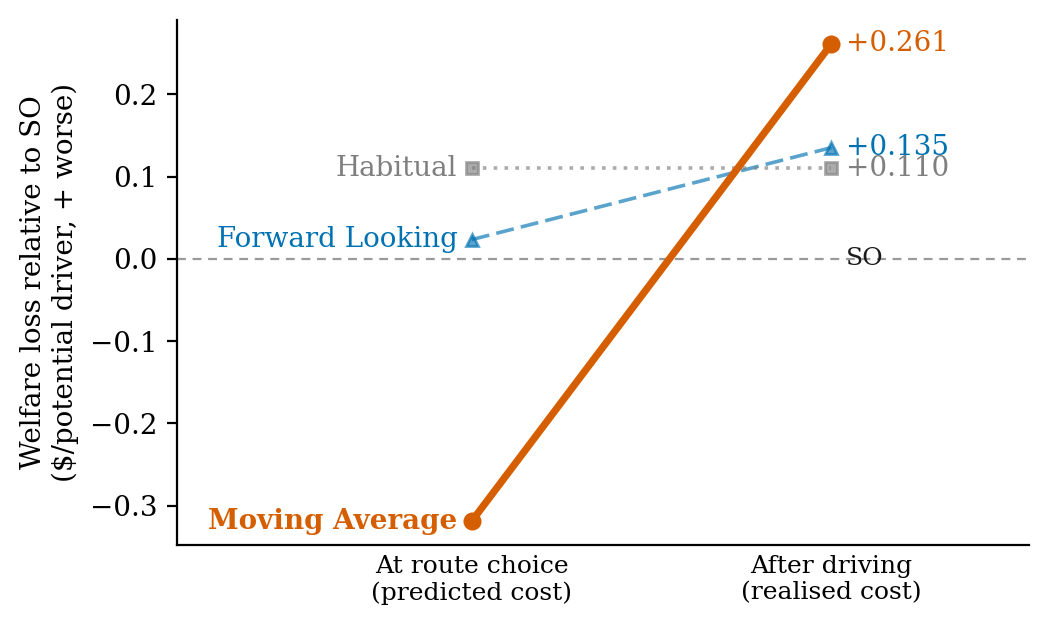
\includegraphics[width=\linewidth]{plot_1_flip.png}
\caption{\textbf{Expected-to-experienced welfare reversal.} Welfare loss by routing rule at zero toll relative to the System Optimum. Values are USD per potential driver. Positive values indicate lower welfare. Expected welfare uses expected costs, while experienced welfare uses realised chosen-route costs.}
\label{fig:flip}
\end{figure}
\FloatBarrier

To illustrate the scale of these differences, the analysis treats the modelled 7.5 km route as one quarter of a 30 km one-way commute and assumes 250 round-trip commuting days per year. This produces an annual multiplier of $4\times2\times250=2{,}000$ modelled-route equivalents per driver. The corresponding illustrative annual welfare losses are approximately USD 523 under Moving Average, USD 271 under Forward Looking, and USD 220 under Habitual. Moving Average exceeds Habitual by approximately USD 303 per driver-year [263, 342], while replacing Moving Average with Forward Looking reduces the illustrative annual loss by approximately USD 252 [214, 286]. These values illustrate scale only and are not forecasts for a particular road or commuter population.

The route-allocation diagnostics help explain the ranking. The standard deviation of the minute-level short-route share is 46 percentage points under Moving Average, 15 under Forward Looking, and 9 under Habitual. Moving Average reacts to recently observed driving times. Many drivers can respond to the same signal before the consequences of their choices become visible in completed observations. This delayed collective response repeatedly moves traffic towards the route that recently appeared less costly. Forward Looking uses the current assigned-route count to anticipate the conditions likely to develop and therefore produces a more stable allocation.

Routing regret provides supporting evidence. Median regret is zero under both adaptive rules, but mean regret is 37 seconds under Moving Average and 24 seconds under Forward Looking. The heavier Moving Average tail indicates that more drivers experience a selected route that is costlier than the estimated alternative. The diagnostic is consistent with the welfare ranking, although it does not by itself establish the cause of the difference.

\begin{figure}[htbp]
\centering
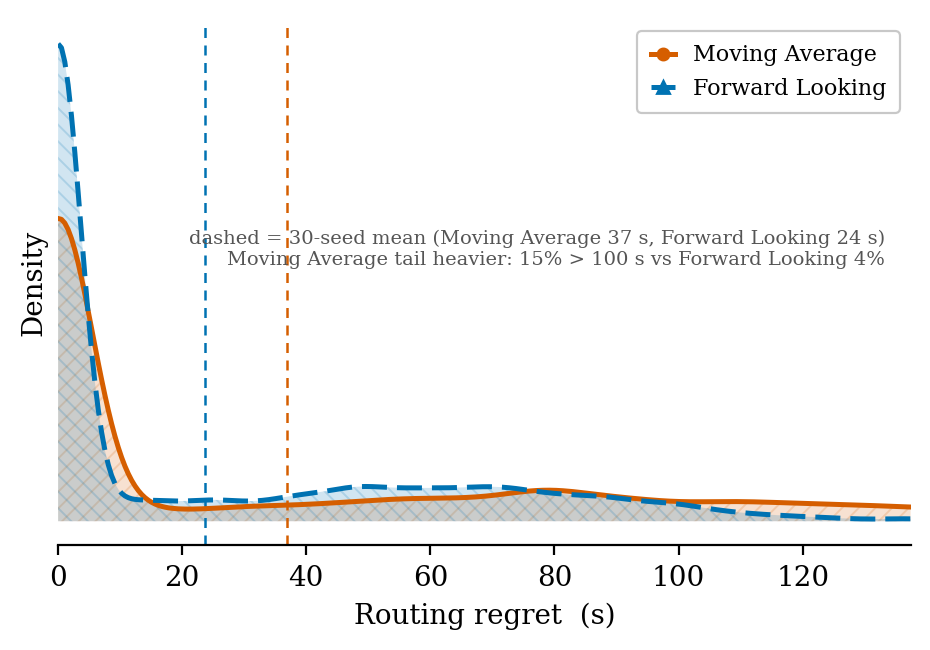
\includegraphics[width=\linewidth]{plot_6b_regret.png}
\caption{\textbf{Routing-regret diagnostic at zero toll.} Dashed lines indicate the 30-seed means for Moving Average (37 s) and Forward Looking (24 s). Moving Average has the heavier right tail.}
\label{fig:regret}
\end{figure}
\FloatBarrier

Tolling changes the remaining welfare loss differently under each routing rule. The largest measured Moving Average improvement occurs at USD 0.50 and reduces welfare loss by USD 0.102 per potential driver [0.082, 0.118]. The largest measured Forward Looking improvement occurs at USD 0.17 and equals USD 0.043 [0.028, 0.057]. The largest measured Habitual improvement occurs at USD 0.28 and equals USD 0.033 [0.017, 0.049]. Under the annual normalization, these reductions equal approximately USD 204, USD 86, and USD 66 per regular driver. Results for every pure routing rule and toll are reported in Annex Table~\ref{tab:pure-rule-grid}.

A higher toll can reverse the welfare effect. At USD 0.50, the toll increases Forward Looking welfare loss by USD 0.026 per potential driver [0.009, 0.044]. This equals approximately USD 53 per regular driver under the annual normalization. The same toll reduces Moving Average loss by approximately USD 204 per regular driver. A price selected for one routing behaviour can therefore become counterproductive when drivers use another.

\begin{figure}[htbp]
\centering
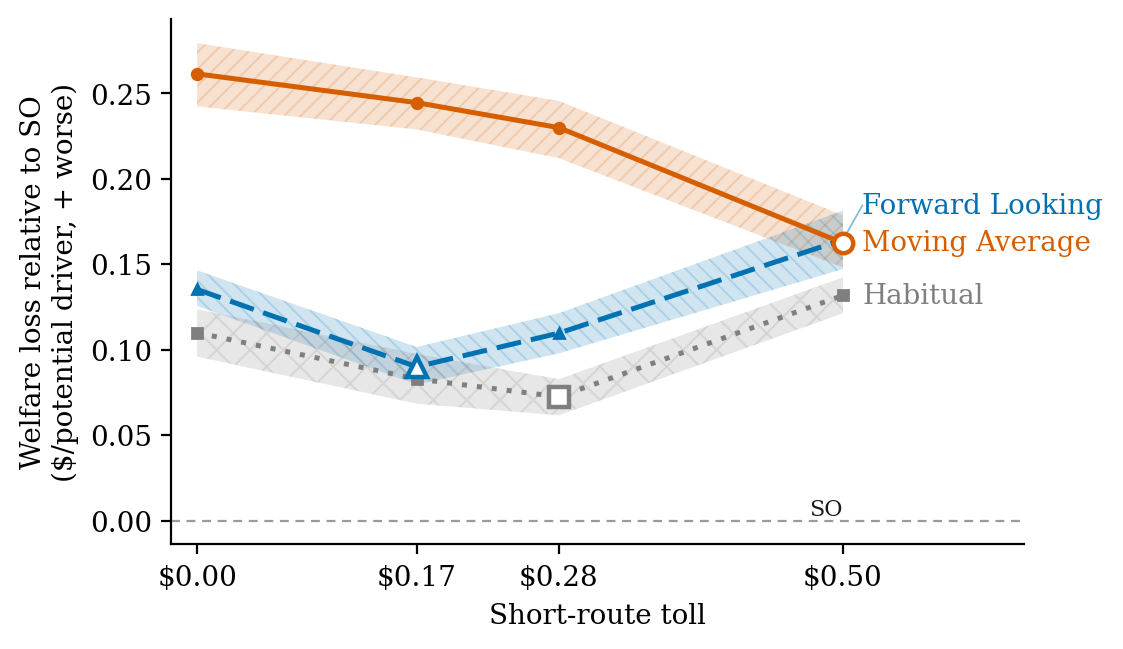
\includegraphics[width=\linewidth]{plot_3_toll_response.png}
\caption{\textbf{Welfare loss under the tested tolls.} Experienced welfare loss is measured relative to the System Optimum at the same toll and expressed in USD per potential driver. Shaded bands show 95\% paired-seed bootstrap confidence intervals based on 1,000 resamples. Hollow markers identify the minimum measured loss on the tested grid.}
\label{fig:toll}
\end{figure}
\FloatBarrier

The no-trip response helps explain why the toll effects differ. At USD 0.50, the share selecting the no-trip alternative rises from 4.9\% to 16.4\% under Moving Average, from 2.5\% to 16.9\% under Forward Looking, and from 5.1\% to 32.2\% under Habitual. Adaptive drivers can respond through both route choice and participation. Habitual drivers cannot change the route assigned by their rule, so a larger share responds by selecting the no-trip alternative. A reduction in congestion may therefore reflect fewer completed drives as well as a different allocation between routes. The welfare measure includes both responses.

\begin{figure}[htbp]
\centering
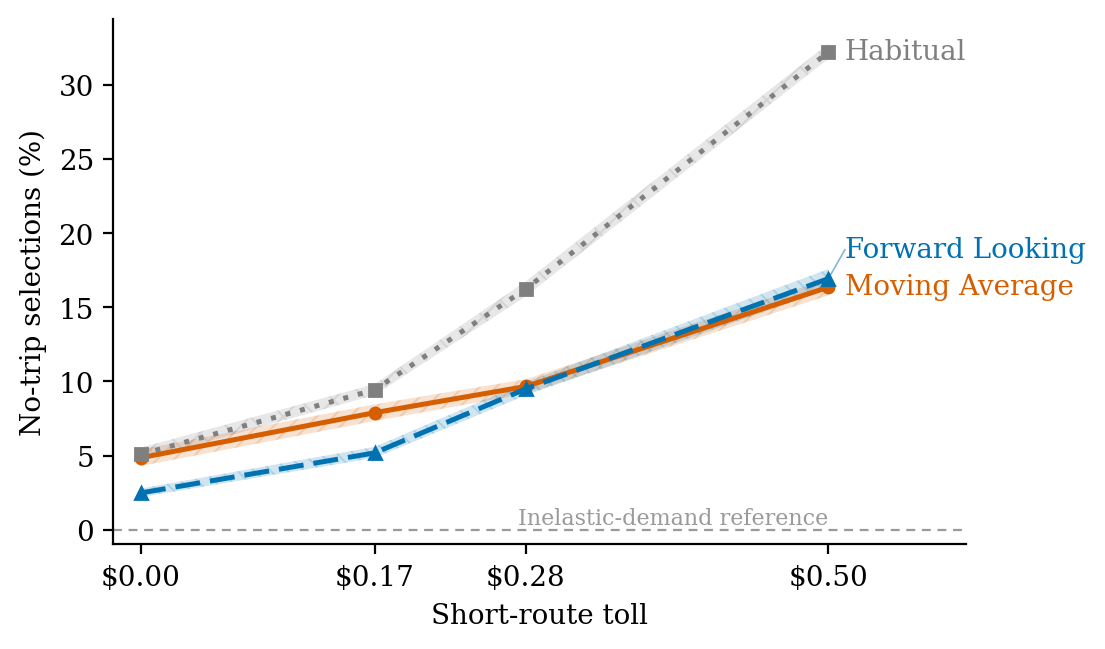
\includegraphics[width=\linewidth]{plot_7_suppression.png}
\caption{\textbf{No-trip selections under tolling.} The figure shows the share of potential drivers selecting the no-trip alternative under each routing rule. Shaded bands are 95\% paired-seed bootstrap confidence intervals based on 1,000 resamples. The dashed zero line is the inelastic-demand reference.}
\label{fig:suppression}
\end{figure}
\FloatBarrier

The participation response is concentrated among drivers with lower values of time. Under Moving Average at USD 0.50, the mean value of time is USD 20.99 per hour among drivers who complete a drive and USD 9.55 among those selecting the no-trip alternative. A fixed monetary toll represents a larger time-equivalent cost for a driver with a lower value of time. This comparison describes which drivers select the no-trip alternative.

\begin{figure}[htbp]
\centering
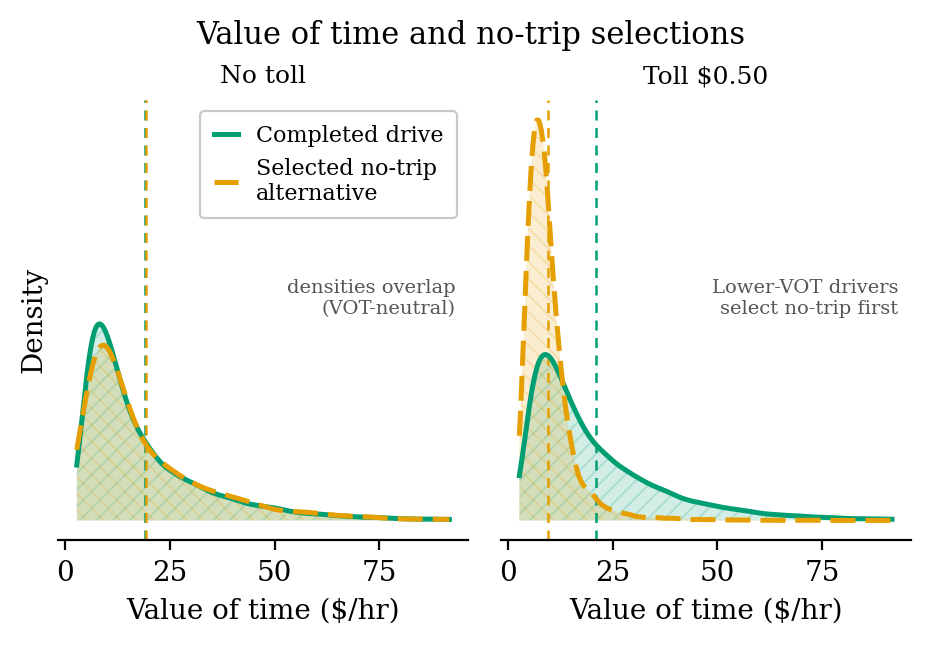
\includegraphics[width=\linewidth]{plot_4_regressivity.png}
\caption{\textbf{Value of time and the no-trip alternative.} Value-of-time densities among drivers completing drives and drivers selecting the no-trip alternative under Moving Average. The distributions overlap without tolling. At \$0.50, no-trip selections are concentrated among drivers with lower values of time. Dashed vertical lines mark the group means.}
\label{fig:regressivity}
\end{figure}
\FloatBarrier

The following three configurations illustrate how routing-rule, toll, and interaction contributions can reinforce or offset one another in determining the remaining experienced welfare loss.

\begin{table}[htbp]
\centering
\footnotesize
\setlength{\tabcolsep}{3pt}
\begin{tabular}{p{0.35\linewidth}rrrr}
\toprule
Evaluated configuration & Routing rule & Toll & Interaction & Remaining loss \\
\midrule
80\% Habitual and 20\% Moving Average at a toll of USD 0.17 & 0.1402 & -0.0230 & -0.0601 & 0.0572 \\
Pure Forward Looking at a toll of USD 0.50 & 0.1353 & 0.0264 & 0.0000 & 0.1617 \\
30\% Forward Looking and 70\% Moving Average at a toll of USD 0.28 & 0.2236 & -0.0255 & -0.1103 & 0.0878 \\
\bottomrule
\end{tabular}
\caption{\textbf{Additive welfare-loss contributions for three evaluated configurations.} Values are USD per potential driver. Positive values increase welfare loss and negative values reduce it.}
\label{tab:additive-examples}
\end{table}

The first configuration has the lowest remaining-loss point estimate among the 176 mixed-population cells. Its toll and interaction contributions offset 59.2\% of the initial routing-rule contribution, and its interaction contribution is USD -0.0601 per potential driver [-0.0732, -0.0475]. The second configuration illustrates the harmful toll effect described above. The third has the largest measured interaction reduction, at USD -0.1103 per potential driver [-0.1234, -0.0954]. These intervals quantify uncertainty around the reported contributions. They do not establish that the first configuration has the lowest true remaining loss or that the third has the largest true interaction reduction among all evaluated cells.

Under the annual normalization, the first configuration has an initial loss of USD 280, a toll contribution of USD -46, an interaction contribution of USD -120, and a remaining loss of USD 114 per regular driver. The remaining loss is USD 323 for pure Forward Looking at a toll of USD 0.50 and USD 176 for the third configuration.

The subgroup decomposition shows who receives the interaction benefit. In the 80\% Habitual and 20\% Moving Average configuration, welfare loss falls by USD 0.1695 per Moving Average driver and USD 0.0327 per Habitual driver relative to their corresponding pure populations at the same toll. After weighting these differences by the population shares, Moving Average accounts for 56.4\% of the interaction reduction and Habitual accounts for 43.6\%. The result therefore does not arise solely because the smaller Moving Average group benefits at the expense of the Habitual majority.

The largest interaction reduction has a different composition. In the population containing 70\% Moving Average and 30\% Forward Looking drivers at a toll of USD 0.28, Moving Average accounts for 99.4\% of the interaction reduction. Forward Looking accounts for the remaining 0.6\%. Its estimated reduction in welfare loss is USD 0.002 per Forward Looking driver [-0.033, 0.034]. The interval spans both a small reduction and a small increase in loss, so the simulations do not identify a clear Forward Looking subgroup effect. The interaction benefit in this configuration is therefore almost entirely associated with Moving Average drivers.

Across the 132 tolled population cells, the toll and population-interaction contributions jointly reduce the initial routing-rule loss in 122 cells. They offset at least half of that loss in 33 cells, although no tested configuration eliminates the loss relative to the zero-toll System Optimum. In 67 cells, population interaction reduces welfare loss by more than the absolute size of the direct toll contribution. The final result should therefore not be attributed to the toll without also considering population composition. Complete remaining-loss and interaction results are reported in Annex Figures~\ref{fig:mixed-remaining-loss} and \ref{fig:population-interaction}, while Annex Table~\ref{tab:best-additive-mix} reports the best tested toll and additive components for every evaluated population composition.

The lowest measured loss occurs in a Habitual-dominated population, although several configurations with larger adaptive shares have similar point estimates. The relationship between adaptive adoption and welfare loss is non-monotonic. Populations with approximately 90\% adaptive adoption have the largest measured losses at the tested tolls. The highest-loss population contains 90\% Moving Average drivers at tolls from USD 0 to USD 0.28 and 90\% Forward Looking drivers at USD 0.50.

This non-monotonic pattern is consistent with evidence that intermediate adoption can moderate the collective response to delayed information, while high adoption can intensify traffic oscillations \parencite{wahleEtAl2002,krallEtAl2021}. The simulations support this pattern within the evaluated grid but do not establish a general adoption threshold.

\begin{figure}[htbp]
\centering
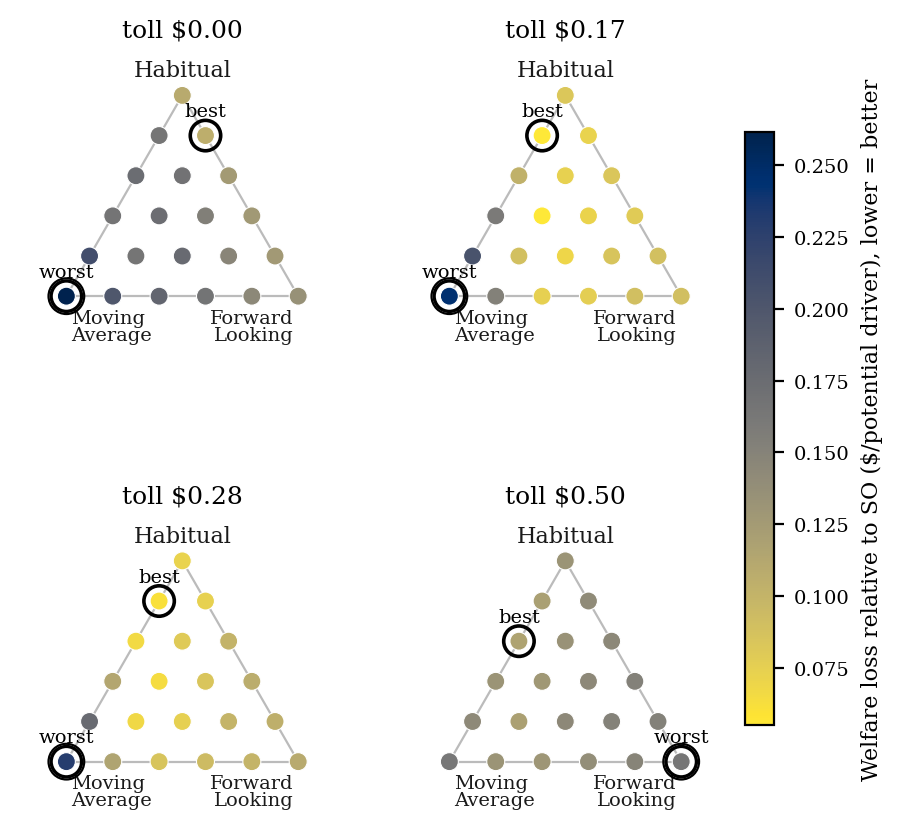
\includegraphics[width=\linewidth]{plot_8_mix_simplex.png}
\caption{\textbf{Welfare loss across population mixes.} Each panel shows the regular 0.20-step simplex at one toll. The corners represent pure Moving Average, Forward Looking, and Habitual populations. Colour denotes experienced welfare loss relative to the System Optimum in USD per potential driver. Lower values indicate better outcomes. Rings mark the sampled grid points with the lowest and highest loss. Targeted off-grid refinements are omitted.}
\label{fig:simplex}
\end{figure}
\FloatBarrier

The point-estimate ordering changes with operating flow. At 3,000 vehicles per hour, welfare loss is USD 0.079 per potential driver under Habitual, USD 0.094 under Forward Looking, and USD 0.266 under Moving Average. This point-estimate order matches the primary semi-congested setting.

At 2,000 vehicles per hour, Moving Average has the lowest point estimate at USD 0.004 per potential driver, followed by Forward Looking at USD 0.018 and Habitual at USD 0.085. However, the paired difference between Moving Average and Forward Looking is not statistically significant. The analysis therefore does not establish which adaptive rule performs better at this flow.

At both lower flows, the best tested System Optimum uses the maximum searched short-route share of 0.55. A higher-welfare allocation may exist beyond this search boundary. If so, the reported welfare losses relative to the System Optimum understate the corresponding gaps. Annex Table~\ref{tab:flow-sensitivity} reports the complete point-estimate comparison.

The flow result is consistent with the curvature of the route-cost relation. When route flow varies around its mean, the additional average cost is approximately $\tfrac{1}{2}c''(\bar f)\operatorname{Var}(f)$. Similar route-share variation has little welfare effect on the flatter free-flow branch and a larger effect where the cost relation steepens near congestion. The simulations therefore establish the adaptive-rule difference in the semi-congested setting but do not establish its direction under free-flow conditions.

The numerical setting shows how the common welfare method distinguishes the effect of a routing rule, the contribution of a toll, and the interaction among routing behaviours. The largest differences arise near the semi-congested operating range, where many drivers responding to a common signal can move congestion between routes. Their magnitude may differ in other networks and behavioural settings.

\clearpage
\section{Conclusion}

At departure, each commuter has a private incentive to select the route with the lowest expected cost. The difference between this private incentive and the network-wide optimum is well established. The contribution of this research is to quantify the welfare consequence of adaptive selfish navigation. In the semi-congested numerical setting, Moving Average offered the lowest expected private cost but produced the highest experienced welfare loss after the collective response was considered. Moving Average produced USD 0.152 more experienced welfare loss per potential driver than the Habitual rule, which represents random route allocation. Under the illustrative commuter normalisation defined in the Numerical Use Case, this difference corresponds to approximately USD 303 per commuter-year. Experienced welfare loss therefore converts the known conflict between individual and network interests into a monetary measure within a defined simulation setting.

The established discussion is commonly framed as a choice between current and lagged information. Previous studies proposed wider observation windows to reduce oscillations by making guidance less responsive \parencite{wahleEtAl2002,krallEtAl2021}. This research reframes the problem as a distinction between backward-looking and forward-looking use of the same recent information. At the moment of prediction, backward-looking observations describe conditions previously encountered by vehicles at the relevant road locations. By the time the recommended commuter reaches those locations, the vehicles that contributed to the estimate have advanced and subsequent route choices have changed traffic flows. A backward-looking method therefore predicts a future driving condition from a past condition that its own recommendations help to change. This timing feedback can produce oscillation. A wider window may weaken the oscillation, but it does not correct the timing mismatch. The findings therefore support moving beyond the trade-off between information freshness and stability by predicting the conditions commuters are likely to encounter.

Forward Looking changes the prediction target from recently observed conditions to conditions likely to be experienced. Following \textcite{davis2009}, it relates current assigned-route counts to subsequently observed driving times. This research applies that principle to two parallel traffic-responsive routes using route-specific expected times. To the best of our knowledge, previous research has not applied Davis’s anticipatory route-count principle to two parallel routes whose driving times both respond to traffic. Extending the method to larger networks remains an important direction for further research.

Population composition creates an additional consequence. Earlier studies found that oscillations intensify when a large share of drivers responds to the same backward-looking information \parencite{wahleEtAl2002,krallEtAl2021}. To the best of our knowledge, previous research has not evaluated experienced welfare in a population combining two adaptive navigation methods with a Habitual population representing random route allocation. In 33 of the 36 evaluated cells that mixed Moving Average and Forward Looking, welfare loss was significantly lower than the share-weighted result predicted from the corresponding pure populations. In the remaining three cells, the difference from the share-weighted prediction was not statistically significant. The relationship between adaptive adoption and welfare loss was nevertheless non-monotonic. The lowest measured loss occurred in a Habitual-dominated population, although several configurations with larger adaptive shares had similar point estimates. Populations with approximately 90\% adaptive adoption had the largest measured losses at the tested tolls. These findings show that mixing navigation methods can moderate welfare loss within the evaluated setting, but they do not establish a general adoption threshold. Because the analysis did not model the decisions or incentives of navigation-application providers, it cannot determine whether they would voluntarily adopt methods that reduce network-wide welfare loss or whether coordination, common standards, or policy incentives would be needed.

Coordinated or mediated routing is a particularly promising direction for future research. A mediator can distribute recommendations across users while preserving their incentives to follow them, rather than improving each commuter's prediction independently \parencite{vassermanEtAl2015}. Recent field evidence shows that small coordinated interventions can improve network conditions \parencite{aroraEtAl2026}. Applying the experienced-welfare method to mediated routing could establish whether these gains persist under partial adoption, heterogeneous values of time, and elastic demand.

This concern may grow if autonomous vehicles consistently follow route guidance \parencite{lentzakisEtAl2018}. Commuters currently add behavioural diversity by following habitual routes or declining an application’s recommendation. Automated routing may reduce this diversity and move the population towards the high-adoption conditions examined in the numerical use case. The consequence will depend on whether future navigation systems are backward-looking, forward-looking, or coordinated. Future research should examine populations using closely related systems with different parameters.

Navigation behaviour changes the welfare effect of a toll within a second-best pricing setting. \Textcite{yang1999} found that route guidance and road pricing can complement one another. The present findings show that the welfare effect of a toll also depends on the navigation systems used by the population. The highest tested toll was USD 0.50 for the 7.5 km route. Under the same illustrative commuter normalisation, this corresponds to a USD 2 toll per 30 km one-way commute. Relative to zero toll, the USD 0.50 toll decreased annual welfare loss by approximately USD 204 per commuter-year under Moving Average and increased it by approximately USD 53 per commuter-year under Forward Looking. The same toll can therefore improve welfare under one navigation method and reduce it under another. A second-best toll should be estimated using current and expected navigation-app adoption and reconsidered when that adoption changes.

\enlargethispage{\baselineskip}
The effectiveness of navigation systems should be assessed not only through total driving time and prediction accuracy, but also through measures that reflect commuter behaviour and experienced outcomes. Experienced welfare loss provides such a measure by incorporating differences in value of time, toll responses, and the decision not to drive. Road authorities should also account for the navigation methods used by commuters when setting tolls. Although the annual monetary estimates remain specific to the defined numerical setting, the transferable contribution is a method for quantifying the welfare consequences of adaptive navigation methods and the interaction between information timing, navigation behaviour, and pricing.

\clearpage
\appendix
\renewcommand{\thetable}{A.\arabic{table}}
\renewcommand{\thefigure}{A.\arabic{figure}}
\setcounter{table}{0}
\setcounter{figure}{0}
\section{Annex}


The annex collects the tables behind the figures and the robustness checks. All quantities are the experienced measure at $\mu = 0.5$ unless stated otherwise, computed by the analysis code over the paired-seed primary dataset.

Traffic was represented microscopically in SUMO version 1.26.0\footnote{SUMO version 1.26.0 is documented in \textcite{sumo2026}.} using a simulation step of 0.2 seconds, following the simulation framework described by \textcite{alvarezLopezEtAl2018}.

The main parameters used to initialise the simulation are summarised in Table M1. Parameters used only in the later construction of experienced costs, welfare, and statistical estimates are introduced in the relevant measurement sections rather than in this table.

\noindent\textbf{Table M1. Simulation initialization parameters}

\begin{center}
\small
\begin{tabular}{@{}p{0.13\textwidth}p{0.25\textwidth}p{0.16\textwidth}p{0.35\textwidth}@{}}
\toprule
\textbf{Symbol} & \textbf{Parameter} & \textbf{Value} & \textbf{Basis} \\
\midrule
$\theta$ & Route-choice logit scale & $0.05\ \mathrm{s}^{-1}$ & Fixed behavioural specification \\
$\mu$ & Route-choice-nest dissimilarity & $0.5$ & Primary elastic-demand specification \\
$\bar Z$ & No-trip reservation cost & $420$ s & Fixed behavioural specification \\
$\mathrm{MCPF}$ & Marginal cost of public funds & $1.2$ & Fixed for all comparisons following \textcite{adlerEtAl2010} \\
$Q^*$ & Total network demand & $3{,}835$ veh/h & Approximately 85\% of the measured short-route forward entry bottleneck, accounting for the 78\% forward share and an even route split. \\
$\alpha$ & Moving Average smoothing factor & $0.1$ & \textcite{davis2009} specification \\
$B$ & Adaptive-rule observation window & $199$ observations per route & Last $B$ observations for each route \\
$u_{\mathrm{ff}}$ & Free-flow speed & $40$ m/s & Network design \\
$L_s$ & Short-route length & $7{,}500$ m & Network design \\
$L_{\ell}$ & Long-route length & $9{,}375$ m & Network design \\
$t_{\min,s}$ & Minimum full-path time, short route & $187.5$ s & Derived \\
$t_{\min,\ell}$ & Minimum full-path time, long route & $234.375$ s & Derived \\
Simulation step & Tactical update interval & $0.2$ s & SUMO configuration \\
Simulation horizon & Total run duration & $7{,}200$ s & Experimental specification \\
Warm-up & Excluded initial period & $3{,}600$ s & Experimental specification \\
\bottomrule
\end{tabular}
\end{center}

The calibrated vehicle settings are reported in Table~\ref{tab:vehicle-parameters}.

\begin{table}[htbp]
\centering
\footnotesize
\setlength{\tabcolsep}{4pt}
\begin{tabular}{@{}p{0.25\textwidth}p{0.25\textwidth}p{0.42\textwidth}@{}}
\toprule
\textbf{Component} & \textbf{Private vehicles} & \textbf{Trucks} \\
\midrule
Traffic share & 97\% & 3\% \\
Microscopic behaviour & Krauss car-following and LC2013 lane changing & Krauss car-following and LC2013 lane changing \\
Vehicle length and minimum gap & 5 m and 1.5 m & 12 m and 2.5 m \\
Assigned maximum speed & Normal distribution with mean 99.5 km/h and standard deviation 10 km/h, then a 5 km/h adjustment and a 60 km/h lower bound & Normal distribution with mean 90 km/h and standard deviation 5 km/h, then a 5 km/h adjustment and bounds of 60 and 95 km/h \\
Following time & Speed dependent from 0 to 3.2 s, calculated as $h_i=3.2-0.055(u_i-80)$ & 1.3 s \\
Driving imperfection & 0.3 & 0.3 \\
Opposing-lane overtaking & Enabled with speed-gain, assertiveness, and impatience parameters of 10, 5, and 1 & Disabled \\
\bottomrule
\end{tabular}
\caption{Vehicle parameters used in the calibrated SUMO setting. The parameters were calibrated jointly to reproduce the intended Van Aerde speed-flow relationship.}
\label{tab:vehicle-parameters}
\end{table}

Table~\ref{tab:measurement-procedures} summarises the treatment of observations that did not provide a directly observed complete-route driving time.

\begin{table}[htbp]
\centering
\footnotesize
\setlength{\tabcolsep}{4pt}
\begin{tabular}{@{}p{0.27\textwidth}p{0.65\textwidth}@{}}
\toprule
\textbf{Observation} & \textbf{Measurement treatment} \\
\midrule
Valid completed drive & The recorded driving time was used when it was at least 187.5 seconds on the short route or 234.375 seconds on the longer alternative. \\
Partial-route observation & A recorded time below the relevant physical minimum indicated mid-route insertion and was not used as a complete-route time. The experienced time was represented by the mean among valid completed drivers departing on the same route during the same 60-second interval. \\
Incomplete drive & A driver still in transit at the end of the analysis window was retained in $\mathcal D$. The complete-route time was represented by the same route and departure-interval mean used for a partial-route observation. \\
Empty departure interval & The nearest earlier populated interval on the same route supplied the complete-route time. The route free-flow time was used when no earlier populated interval was available. \\
Queued driver & A driver unable to enter the assigned route before the analysis ended was retained in $\mathcal D$. Projected driving time combined waiting time from the planned departure with the assigned-route length divided by the projection-floor speed of 16.44 m/s. \\
Unselected route for regret & The counterfactual route cost used the valid completed-route mean for the corresponding route and 60-second departure interval, with the same empty-interval rule. \\
\bottomrule
\end{tabular}
\caption{Treatment of full-route validity, incomplete drives, and counterfactual route costs. The same rules were applied across all evaluated cells.}
\label{tab:measurement-procedures}
\end{table}

The model deliberately isolates route-choice, information, and tolling mechanisms. It does not attempt to represent every component of transport demand or welfare.

\begin{center}
\small
\begin{tabular}{@{}p{0.24\textwidth}p{0.68\textwidth}@{}}
\toprule
\textbf{Excluded component} & \textbf{Scope decision} \\
\midrule
Schedule delay & Departure timing is exogenous, and no early- or late-arrival utility is modelled. \\
Mode choice & The experiment contains one transport mode and a drive or no-trip margin only. \\
Environmental externalities & Emissions and other environmental effects are outside the welfare account. Their inclusion could affect welfare levels and potentially cross-treatment comparisons where trip participation differs. \\
Multiple origins and destinations & The parallel-route network isolates the mechanism under study. More complex network structures are left for future work. \\
Braess-type network effects & The study does not vary network topology or examine paradoxes created by adding links. \\
Coordinated or mediated routing & Drivers respond individually to the specified routing rules. A central mechanism coordinating recommendations across users is not modelled. \\
Information-provision interventions & The experiment does not vary whether information is provided or withheld. It compares the specified navigation-rule architectures operating within the same simulated environment. \\
Full parameter estimation & Behavioural parameters are fixed as part of the experimental specification rather than estimated from individual choice data. \\
\bottomrule
\end{tabular}
\end{center}

The System Optimum split was identified by evaluating five short-route shares at the primary operating point and zero toll.

\begin{table}[htbp]
\centering
\small
\setlength{\tabcolsep}{4pt}
\begin{tabular}{ccc}
\toprule
\shortstack{Short-route\\share $p$} & \shortstack{Additional welfare loss\\relative to best (\$/potential driver)} & \shortstack{$n$\\seeds} \\
\midrule
0.40 & 0.0124 & 30 \\
0.45 & 0.0000 & 30 \\
0.50 & 0.0102 & 30 \\
0.55 & 0.0538 & 30 \\
0.60 & 0.1668 & 30 \\
\bottomrule
\end{tabular}
\caption{System Optimum split search at $Q^*=3{,}835$ veh/h. Positive values indicate lower experienced welfare than the best tested allocation.}
\label{tab:so-split-profile}
\end{table}

Table~\ref{tab:flip} reports the two consumer-surplus measures behind Figure~\ref{fig:flip}.

\begin{table}[htbp]
\centering
\footnotesize
\setlength{\tabcolsep}{3pt}
\begin{tabular}{lccc}
\toprule
Rule & \shortstack{Expected difference\\from SO (\$/potential driver)} & \shortstack{Experienced loss\\relative to SO (\$/potential driver)} & \shortstack{$n$\\seeds} \\
\midrule
System Optimum & 0.000 & 0.000 & 30 \\
Moving Average & $-0.319$ & 0.261 [0.242, 0.279] & 30 \\
Forward Looking & 0.023 & 0.135 [0.126, 0.146] & 30 \\
Habitual & 0.110 & 0.110 [0.096, 0.124] & 30 \\
\bottomrule
\end{tabular}
\caption{Expected and experienced welfare differences at zero toll. A positive value indicates lower welfare than the System Optimum. Brackets contain the 95\% paired-seed confidence interval for experienced loss.}
\label{tab:flip}
\end{table}

The master table reports experienced welfare loss relative to the System Optimum at the same toll, the direct toll effect relative to each rule's zero-toll condition, the share selecting the no-trip alternative, and the number of seeds.

\begin{table}[htbp]
\centering
\small
\setlength{\tabcolsep}{4pt}
\begin{tabular}{lccccc}
\toprule
Rule & Toll & \shortstack{Loss relative\\to SO} & \shortstack{Direct toll\\effect} & \shortstack{No-trip\\share} & \shortstack{$n$\\seeds} \\
\midrule
Moving Average & 0.00 & 0.261 & 0.000 & 4.9\% & 30 \\
Moving Average & 0.17 & 0.245 & 0.015 & 7.9\% & 30 \\
Moving Average & 0.28 & 0.230 & 0.027 & 9.7\% & 30 \\
Moving Average & 0.50 & 0.162 & 0.102 & 16.4\% & 30 \\
Forward Looking & 0.00 & 0.135 & 0.000 & 2.5\% & 30 \\
Forward Looking & 0.17 & 0.090 & 0.043 & 5.2\% & 30 \\
Forward Looking & 0.28 & 0.110 & 0.021 & 9.5\% & 30 \\
Forward Looking & 0.50 & 0.164 & $-0.026$ & 16.9\% & 30 \\
Habitual & 0.00 & 0.110 & 0.000 & 5.1\% & 30 \\
Habitual & 0.17 & 0.083 & 0.025 & 9.4\% & 30 \\
Habitual & 0.28 & 0.072 & 0.033 & 16.3\% & 30 \\
Habitual & 0.50 & 0.132 & $-0.019$ & 32.2\% & 30 \\
\bottomrule
\end{tabular}
\caption{Pure-rule results at $\mu = 0.5$. Welfare differences are USD per potential driver. A positive direct toll effect indicates a welfare gain relative to the same rule at zero toll.}
\label{tab:pure-rule-grid}
\end{table}

Robustness to the nest-dissimilarity parameter was assessed by re-running Moving Average and Forward Looking at $\mu \in \{0.3, 0.5, 0.7, 1.0\}$ and zero toll. Moving Average's experienced welfare loss relative to Forward Looking ranges from \$0.125 to \$0.130 per potential driver. The System Optimum and Habitual were run only at $\mu = 0.5$. The full four-rule ordering is therefore established at $\mu = 0.5$, while the parameter sweep applies only to the adaptive-rule comparison.

Under SUMO's calibrated free-position insertion rule, a vehicle may enter beyond the route entrance when congestion prevents insertion at the beginning. Its recorded time then covers only part of the route. Such partial-route observations account for 22.4\% of completed Moving Average drives and 8.2\% of completed Forward Looking drives. The higher Moving Average rate is consistent with its larger minute-level route-share variation, although the simulations do not isolate this relationship causally. The full-path correction was therefore tested using alternative same-route replacement values. Replacing these observations with the same-route departure-minute mean, the forward-only mean, or the 25th, 50th, or 75th percentile left Moving Average with between \$0.126 and \$0.136 more welfare loss per potential driver than Forward Looking. A separate diagnostic using only valid direct observations also found a larger prediction-related loss under Moving Average. The relative result is therefore not generated by the selected replacement value.

\begin{table}[htbp]
\centering
\small
\setlength{\tabcolsep}{5pt}
\begin{tabular}{ccc}
\toprule
$\mu$ & \shortstack{Moving Average loss relative to\\Forward Looking (\$/potential driver)} & \shortstack{$n$\\seeds} \\
\midrule
0.3 & 0.125 & 30 \\
0.5 & 0.126 & 30 \\
0.7 & 0.126 & 30 \\
1.0 & 0.130 & 30 \\
\bottomrule
\end{tabular}
\caption{Adaptive-rule welfare difference across the nest-dissimilarity parameter at zero toll. Moving Average retains greater experienced welfare loss than Forward Looking at every tested value.}
\label{tab:mu-sensitivity}
\end{table}

Robustness to the operating point was assessed by re-running the four pure rules at lower network flows. The System Optimum split was re-optimised at each flow. Moving Average has a welfare loss of \$0.266 per potential driver at 3,000 vehicles per hour and \$0.004 at 2,000 vehicles per hour. This supports a regime-dependent interpretation. At 3,000 vehicles per hour, the point-estimate order matches the primary flow.

At 2,000 veh/h, Moving Average has the lowest adaptive-rule point estimate, but its difference from Forward Looking is not statistically resolved. Habitual has the largest loss. At both lower flows, the System Optimum occurs at the upper searched short-route share of 0.55. A wider search could identify a higher-welfare allocation, so the reported welfare losses may be conservative.

\begin{table}[htbp]
\centering
\footnotesize
\setlength{\tabcolsep}{4pt}
\begin{tabular}{ccccc}
\toprule
\shortstack{Flow\\(veh/h)} & \shortstack{System\\Optimum} & Habitual & \shortstack{Forward\\Looking} & \shortstack{Moving\\Average} \\
\midrule
2{,}000 & 0.000 & 0.085 & 0.018 & 0.004 \\
3{,}000 & 0.000 & 0.079 & 0.094 & 0.266 \\
3{,}835 (primary) & 0.000 & 0.110 & 0.135 & 0.261 \\
\bottomrule
\end{tabular}
\caption{Operating-point robustness measured as experienced welfare loss relative to the System Optimum at zero toll. Values are USD per potential driver. At the two lower flows, the welfare-optimal split lies at the top of the searched range of 0.55, so the reported losses are conservative.}
\label{tab:flow-sensitivity}
\end{table}

Population-mix interaction is evaluated relative to the share-weighted additive prediction defined in the Methodology. Of the 176 mixture-and-toll combinations, 104 are below the additive benchmark, 67 are consistent with it, and 5 are above it.

Figures~\ref{fig:mixed-remaining-loss} and~\ref{fig:population-interaction} extend the population comparison across all four toll levels. Table~\ref{tab:best-additive-mix} reports the additive components at the best measured toll for each population composition.

\begin{figure}[p]
\centering
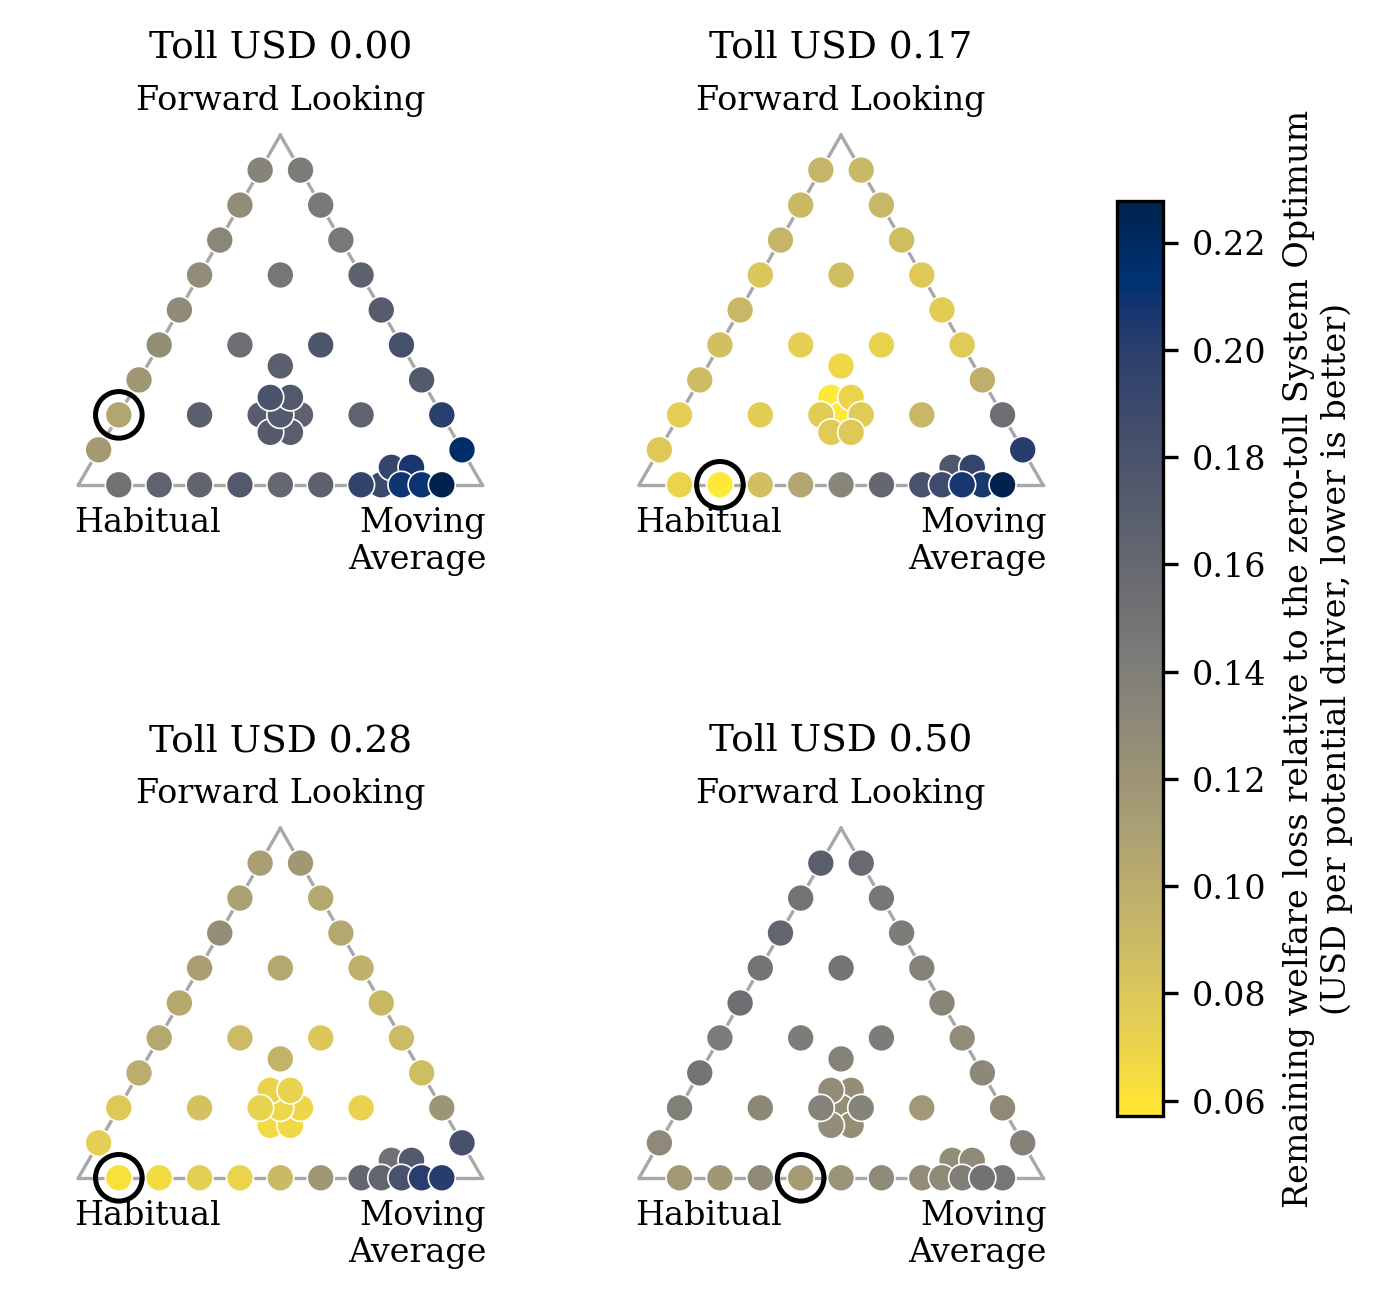
\includegraphics[width=\linewidth]{mixed-remaining-welfare-loss.png}
\caption{Remaining experienced welfare loss across all 176 population-and-toll cells. Every cell is measured relative to the zero-toll System Optimum. Lower values indicate lower remaining welfare loss. Rings identify the lowest-loss composition at each toll.}
\label{fig:mixed-remaining-loss}
\end{figure}

\begin{figure}[p]
\centering
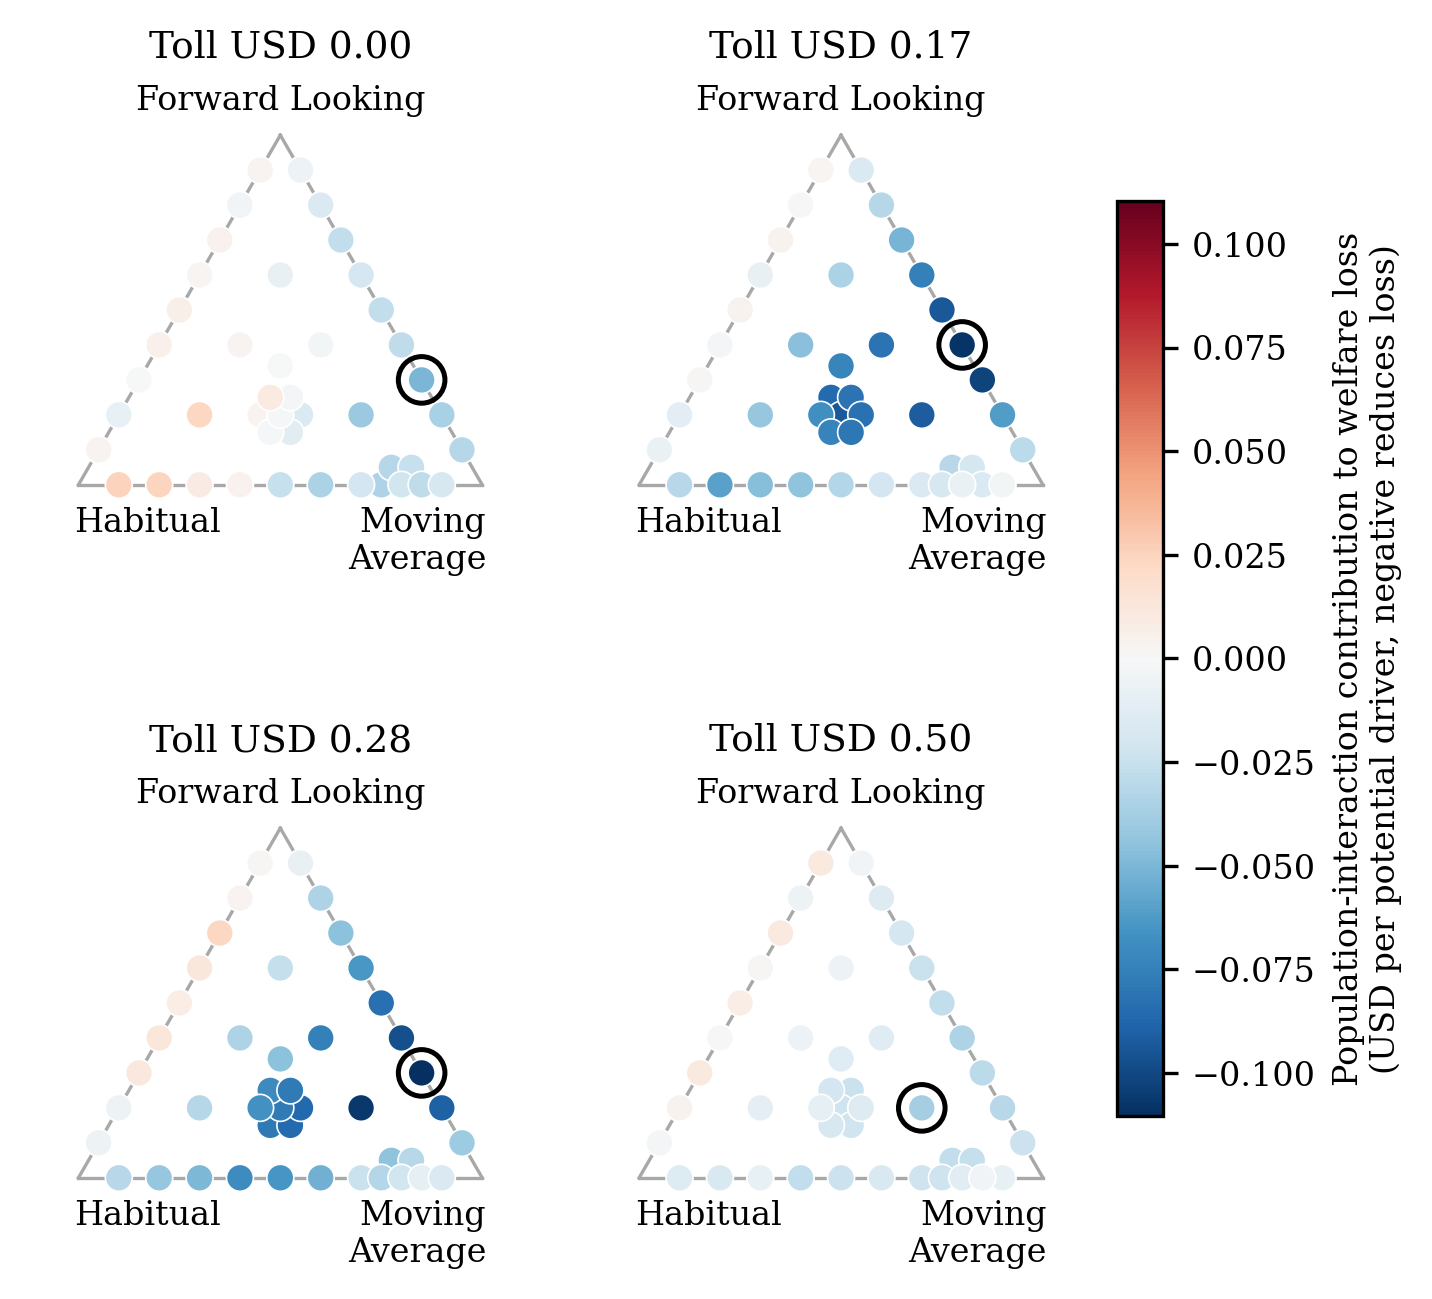
\includegraphics[width=\linewidth]{population-interaction-contribution.png}
\caption{Population-interaction contribution across all 176 population-and-toll cells. Negative values indicate that interaction reduces welfare loss relative to the share-weighted additive prediction. Rings identify the largest loss reduction at each toll.}
\label{fig:population-interaction}
\end{figure}

\clearpage
\begin{landscape}
\pagestyle{empty}
\LandscapePageNumber
\footnotesize
\setlength{\tabcolsep}{3.5pt}
\begin{longtable}{cccccccc}
\caption{Best measured toll and additive decomposition for each mixed population. The best measured toll minimises the remaining welfare-loss point estimate within the evaluated toll grid. Positive components increase welfare loss and negative components reduce it. Values are USD per potential driver. Rows are ordered by remaining welfare loss.}
\label{tab:best-additive-mix}\\
\toprule
\shortstack{Forward\\Looking} &
\shortstack{Moving\\Average} &
Habitual &
\shortstack{Best\\toll} &
\shortstack{Routing-rule\\contribution} &
\shortstack{Toll\\contribution} &
\shortstack{Interaction\\contribution} &
\shortstack{Remaining\\welfare loss} \\
\midrule
\endfirsthead
\multicolumn{8}{c}{Table~\thetable\ continued} \\
\toprule
\shortstack{Forward\\Looking} &
\shortstack{Moving\\Average} &
Habitual &
\shortstack{Best\\toll} &
\shortstack{Routing-rule\\contribution} &
\shortstack{Toll\\contribution} &
\shortstack{Interaction\\contribution} &
\shortstack{Remaining\\welfare loss} \\
\midrule
\endhead
\midrule
\multicolumn{8}{r}{Continued on the next page} \\
\endfoot
\bottomrule
\endlastfoot
0\% & 20\% & 80\% & 0.17 & 0.140 & -0.023 & -0.060 & 0.057 \\
25\% & 35\% & 40\% & 0.17 & 0.169 & -0.026 & -0.086 & 0.057 \\
20\% & 40\% & 40\% & 0.17 & 0.176 & -0.025 & -0.093 & 0.058 \\
0\% & 10\% & 90\% & 0.28 & 0.125 & -0.033 & -0.030 & 0.062 \\
15\% & 40\% & 45\% & 0.28 & 0.174 & -0.029 & -0.079 & 0.066 \\
15\% & 45\% & 40\% & 0.28 & 0.182 & -0.029 & -0.085 & 0.068 \\
34\% & 33\% & 33\% & 0.17 & 0.169 & -0.028 & -0.072 & 0.068 \\
20\% & 45\% & 35\% & 0.28 & 0.183 & -0.028 & -0.086 & 0.069 \\
25\% & 40\% & 35\% & 0.17 & 0.177 & -0.026 & -0.081 & 0.070 \\
0\% & 40\% & 60\% & 0.28 & 0.171 & -0.031 & -0.070 & 0.070 \\
40\% & 40\% & 20\% & 0.17 & 0.181 & -0.028 & -0.081 & 0.071 \\
20\% & 60\% & 20\% & 0.28 & 0.206 & -0.027 & -0.107 & 0.072 \\
20\% & 35\% & 45\% & 0.28 & 0.168 & -0.029 & -0.067 & 0.072 \\
40\% & 20\% & 40\% & 0.17 & 0.150 & -0.030 & -0.046 & 0.074 \\
0\% & 30\% & 70\% & 0.28 & 0.155 & -0.031 & -0.050 & 0.074 \\
10\% & 0\% & 90\% & 0.28 & 0.112 & -0.032 & -0.006 & 0.075 \\
20\% & 0\% & 80\% & 0.17 & 0.115 & -0.029 & -0.011 & 0.075 \\
50\% & 50\% & 0\% & 0.17 & 0.198 & -0.029 & -0.094 & 0.075 \\
20\% & 20\% & 60\% & 0.17 & 0.145 & -0.027 & -0.043 & 0.076 \\
40\% & 60\% & 0\% & 0.17 & 0.211 & -0.026 & -0.108 & 0.077 \\
60\% & 40\% & 0\% & 0.17 & 0.186 & -0.032 & -0.075 & 0.079 \\
60\% & 0\% & 40\% & 0.17 & 0.125 & -0.036 & -0.009 & 0.081 \\
40\% & 0\% & 60\% & 0.17 & 0.120 & -0.032 & -0.002 & 0.086 \\
60\% & 20\% & 20\% & 0.17 & 0.155 & -0.034 & -0.034 & 0.087 \\
70\% & 30\% & 0\% & 0.17 & 0.173 & -0.035 & -0.051 & 0.087 \\
30\% & 70\% & 0\% & 0.28 & 0.224 & -0.025 & -0.110 & 0.088 \\
30\% & 0\% & 70\% & 0.17 & 0.118 & -0.030 & 0.001 & 0.088 \\
0\% & 50\% & 50\% & 0.28 & 0.186 & -0.030 & -0.065 & 0.090 \\
90\% & 10\% & 0\% & 0.17 & 0.148 & -0.040 & -0.017 & 0.091 \\
80\% & 0\% & 20\% & 0.17 & 0.130 & -0.040 & 0.000 & 0.091 \\
80\% & 20\% & 0\% & 0.17 & 0.160 & -0.038 & -0.031 & 0.092 \\
50\% & 0\% & 50\% & 0.17 & 0.123 & -0.034 & 0.003 & 0.092 \\
90\% & 0\% & 10\% & 0.17 & 0.133 & -0.041 & 0.002 & 0.093 \\
70\% & 0\% & 30\% & 0.17 & 0.128 & -0.038 & 0.004 & 0.094 \\
0\% & 60\% & 40\% & 0.28 & 0.201 & -0.030 & -0.053 & 0.118 \\
20\% & 80\% & 0\% & 0.28 & 0.236 & -0.026 & -0.090 & 0.120 \\
5\% & 75\% & 20\% & 0.50 & 0.225 & -0.071 & -0.027 & 0.126 \\
0\% & 70\% & 30\% & 0.50 & 0.216 & -0.065 & -0.023 & 0.128 \\
5\% & 80\% & 15\% & 0.50 & 0.232 & -0.077 & -0.027 & 0.129 \\
0\% & 75\% & 25\% & 0.50 & 0.224 & -0.071 & -0.023 & 0.129 \\
10\% & 90\% & 0\% & 0.50 & 0.249 & -0.089 & -0.023 & 0.137 \\
0\% & 80\% & 20\% & 0.50 & 0.231 & -0.077 & -0.013 & 0.141 \\
0\% & 90\% & 10\% & 0.50 & 0.246 & -0.090 & -0.009 & 0.147 \\
0\% & 85\% & 15\% & 0.50 & 0.239 & -0.084 & -0.004 & 0.151 \\
\end{longtable}
\end{landscape}
\ClearShipoutPictureFG
\pagestyle{plain}

Each reported cell contains 30 valid replications. Paired comparisons use 30 common valid seeds in ascending seed order.

The best measured toll for each rule is the tested value that maximises experienced welfare under that rule. Each welfare-difference interval is the 2.5th to 97.5th percentile of matched-seed bootstrap differences. Sample sizes per condition are listed in the master table.

\clearpage
\printbibliography[title={References}]

\end{document}
